\documentclass[a4, 11pt]{article}

\usepackage{microtype}
%\usepackage[T1]{fontenc} % dejar solo para html
\usepackage[latin1]{inputenc}

\textwidth = 6.5 in 
\textheight = 9 in 
\oddsidemargin = 0.0 in
\evensidemargin = 0.0 in 
\topmargin = 0.0 in
\headheight = 0.0 in 
\headsep = 0.0 in
\parindent = 0.3in
\parskip=10pt
 
\usepackage{graphicx}
\graphicspath{{Fotos/}}

\usepackage{amsmath}
\usepackage{amsfonts}
\usepackage{harmony}
\usepackage{enumerate}
\usepackage{enumitem}
\usepackage{bm}
\usepackage{upgreek}
\usepackage{cancel}

%% ddphonism
% 
% (c) Celia Rubio Madrigal
%
%% This program can be redistributed and/or modified under the terms
%% of the LaTeX Project Public License Distributed from CTAN archives
%% in directory macros/latex/base/lppl.txt.
 
\NeedsTeXFormat{LaTeX2e}
\ProvidesPackage{ddphonism}
[2019/08/10 v0.2 Dodecaphonic diagrams: twelve-tone matrices, clock diagrams, etc.]

\RequirePackage{etoolbox}
\RequirePackage{xparse}
\RequirePackage{tikz}
\RequirePackage{xstring}
\RequirePackage{pgfkeys}


%%%%%%%%%%%%%%%%%%%%%%%%%%%%%%%%%%%%
% Matrices

\usetikzlibrary{matrix}

\ExplSyntaxOn
\DeclareExpandableDocumentCommand{\Evaluation}{m}{\int_eval:n {#1}}
\ExplSyntaxOff

\newcounter{Dsize}
\newcommand{\DsizeMake}[1]{%
	\setcounter{Dsize}{0}%
	\foreach \n in {#1}{%
		\stepcounter{Dsize}%
	}%
}

% Only with numbers.
\newcounter{Dfirst}
\newcommand{\DheadMake}[1]{%
	\setcounter{Dfirst}{-1}%
	\foreach \n in {#1}{%
		\ifnum\theDfirst=-1%
		\setcounter{Dfirst}{\n}%
		\fi%
	}%
}

% Only when DsizeMake is already done.
\newcounter{Dmod}
\newcommand{\Modulo}[1]{%
	\setcounter{Dmod}{#1}%
	\loop%
	\ifnum\theDmod>\Evaluation{\theDsize-1}%		
		\setcounter{Dmod}{\Evaluation{\theDmod-\theDsize}}%
		\repeat%
	\ifnum\theDmod<0%
		\setcounter{Dmod}{\Evaluation{\theDmod+\theDsize}}%
		\repeat%
	\theDmod%
}

\newif\ifdmatrixLines
\newif\ifdmatrixOutside
\newif\ifdmatrixInside
\newif\ifdmatrixV
\newif\ifdmatrixH
\newif\ifdmatrixTikz
\pgfkeys{
	/dmatrix/.is family
	, /dmatrix
	, default/.style = 
		{ lines = false
		, outside lines = false
		, inside lines = false
		, sep = 1
		, vsep = 1
		, hsep = 1
		, no tikz = false
		}
	, no tikz/.is if=dmatrixTikz
	, lines/.is if=dmatrixLines
	, outside lines/.is if=dmatrixOutside
	, inside lines/.is if=dmatrixInside
	, vlines/.is if=dmatrixV
	, hlines/.is if=dmatrixH
	, sep/.estore in=\dmatrixSep
	, vsep/.estore in=\dmatrixVsep
	, hsep/.estore in=\dmatrixHsep
}

\newcommand{\DLOH}{%
	\draw (0.05*\dmatrixSep*\dmatrixHsep,0) --%
	(\theDsize*\dmatrixSep*\dmatrixHsep+0.05*\dmatrixSep*\dmatrixHsep,0);%
	\draw (0.05*\dmatrixSep*\dmatrixHsep,-\theDsize*0.5*\dmatrixSep*\dmatrixVsep) -- %
	(\theDsize*\dmatrixSep*\dmatrixHsep+0.05*\dmatrixSep*\dmatrixHsep,-\theDsize*0.5*\dmatrixSep*\dmatrixVsep);%
}

\newcommand{\DLOV}{%
	\draw (0.05*\dmatrixSep*\dmatrixHsep,0) -- %
	(0.05*\dmatrixSep*\dmatrixHsep,-\theDsize*0.5*\dmatrixSep*\dmatrixVsep);%
	\draw (\theDsize*\dmatrixSep*\dmatrixHsep+0.05*\dmatrixSep*\dmatrixHsep,0) -- %
	(\theDsize*\dmatrixSep*\dmatrixHsep+0.05*\dmatrixSep*\dmatrixHsep,-\theDsize*0.5*\dmatrixSep*\dmatrixVsep);
}

\newcommand{\DLIH}{%
	\draw (0.05*\dmatrixSep*\dmatrixHsep,-\xD*0.5*\dmatrixSep*\dmatrixVsep) -- %
	(\theDsize*\dmatrixSep*\dmatrixHsep+0.05*\dmatrixSep*\dmatrixHsep,-\xD*0.5*\dmatrixSep*\dmatrixVsep);%
}

\newcommand{\DLIV}{%
	\draw (\xD*\dmatrixSep*\dmatrixHsep+0.05*\dmatrixSep*\dmatrixHsep,0) -- %
	(\xD*\dmatrixSep*\dmatrixHsep+0.05*\dmatrixSep*\dmatrixHsep,-\theDsize*0.5*\dmatrixSep*\dmatrixVsep);%
}

\newcommand{\dmatrix}[2][]{%
	\DsizeMake{#2}%
	\DheadMake{#2}%
	%
	\pgfkeys{/dmatrix, default, #1}%
	%
	\ifdmatrixTikz\else%
	\begin{tikzpicture}%
	\fi%
	\foreach [count=\nj] \j in {#2} {%
		\foreach [count=\ni] \i in {#2} {%
			\draw node at 
			( \ni*\dmatrixSep*\dmatrixHsep-0.5*\dmatrixSep*\dmatrixHsep
			, -\nj*\dmatrixSep*\dmatrixVsep/2+0.25*\dmatrixSep*\dmatrixVsep) {%
				\Modulo{\Evaluation{\i-\j+\theDfirst}}%
			};%
		}%
	}%
	\foreach \xD in {1,...,\Evaluation{\theDsize-1}} {%
		\ifdmatrixLines
		\DLOH\DLOV\DLIH\DLIV
		\fi
		\ifdmatrixOutside
		\DLOH\DLOV
		\fi
		\ifdmatrixInside
		\DLIH\DLIV
		\fi
		\ifdmatrixH
		\DLOH\DLIH
		\fi
		\ifdmatrixV
		\DLOV\DLIV
		\fi
	}%
%
\ifdmatrixTikz\else%
\end{tikzpicture}%
\fi%
}


%%%%%%%%%%%%%%%%%%%%%%%%%%%%%%%%%%%%
% Diagrams

\usetikzlibrary{shapes,arrows,decorations.markings,shapes.misc}

\tikzstyle ddiagramArrow=[decoration=
		{markings,mark=at position 0.25 with
			{\arrow[scale=1.25,>=triangle 45]{>}}},
	postaction={decorate}]

\tikzstyle{ddiagram}=[minimum height=0pt,inner sep=0pt,outer sep=0pt,scale=0.65]

\newif\ifddiagramTikz
\pgfkeys{
	/ddiagram/.is family
	, /ddiagram
	, default/.style = 
		{ name =\empty%
		, up =\empty%
		, no tikz = false
		}
	, no tikz/.is if=ddiagramTikz
	, name/.estore in=\ddiagramName
	, up/.estore in=\ddiagramUp
}

\newcounter{Dprev}
\newcommand{\Dvar}{}
\newcommand{\ddiagram}[2][]{%
	\DsizeMake{#2}%
	\DheadMake{#2}%
	%
	\pgfkeys{/ddiagram, default, #1}%
	%
	\ifdefequal{\ddiagramUp}{\empty}%
	{\renewcommand{\Dvar}{\theDfirst}}% if empty
	{\renewcommand{\Dvar}{\ddiagramUp}}% if not empty
	%
	\ifddiagramTikz\else%
	\begin{tikzpicture}[ddiagram,rotate=360*\Dvar/\theDsize]%
	\fi%
	\foreach \x in {0,...,\Evaluation{\theDsize-1}} {%
		\node at (90-360*\x/\theDsize:2) {\x};%
		\node (\x) at (90-360*\x/\theDsize:1.6) {};%
	};%
	%
	\setcounter{Dprev}{-1}%
	\foreach \x in {#2}{%
		\ifnum \theDprev=\theDfirst%
		\draw [style=ddiagramArrow] (\theDprev) -- (\x);%
		\else \ifnum \theDprev=-1%
		\else%
		\draw (\theDprev) -- (\x);%
		\fi\fi%
		\setcounter{Dprev}{\x}%
	};%
	\draw (\theDprev) -- (\theDfirst);%
	%
	\ifdefequal{\ddiagramName}{\empty}%
	{}% if empty
	{\node at (0,0) [circle,fill=white] {\ddiagramName};}% if not empty
	\ifddiagramTikz\else%
	\end{tikzpicture}%
	\fi%
}


%%%%%%%%%%%%%%%%%%%%%%%%%%%%%%%%%%%%
% Dihedral diagrams

\tikzstyle ddihedralArrow=[decoration=
		{markings,mark=at position 1 with {\arrow[scale=1.5,>=angle 60]{>}}},
	postaction={decorate}]

\tikzstyle{ddihedral}=[inner sep=0,minimum height=18pt]

\newif\ifddihedralTikz
\pgfkeys{
	/ddihedral/.is family, /ddihedral,
	default/.style = {t = 0, c = 0, s = 0, v = 0, no tikz=false},
	no tikz/.is if=ddihedralTikz,
	t/.estore in = \ddihedralT,
	c/.estore in = \ddihedralC,
	s/.estore in = \ddihedralS,
	v/.estore in = \ddihedralV,
}

\newif\ifdarrowsTikz
\pgfkeys{
	/darrows/.is family, /darrows,
	default/.style = {no tikz=false},
	no tikz/.is if=darrowsTikz,
}
\newcommand{\darrows}[2][]{%
	\DsizeMake{#2}%
	%
	\pgfkeys{/darrows, default, #1}%
	%
	\ifdarrowsTikz\else%
	\begin{tikzpicture}%
	\fi%
	\draw foreach \x in {0,...,\Evaluation{\theDsize-1}} {%
		(90-360*\x/\theDsize:2.5) node[circle] (\x) {}%
	};%
	\foreach \x [count=\y] in {#2} {%
		\draw [style=ddihedralArrow] (90-360*\Evaluation{\y-1}/\theDsize:1.25) -- (\x);%
	};%
	\ifdarrowsTikz\else%
	\end{tikzpicture}%
	\fi%
}

\newcommand\ddihedral[2][]{%
	\DsizeMake{#2}%
	%
	\pgfkeys{/ddihedral, default, #1}%
	%
	\ifddihedralTikz\else%
	\begin{tikzpicture}[ddihedral]%
	\fi%
	\draw foreach \x in {0,...,\Evaluation{\theDsize-1}} {%
		(\Evaluation{(90+\ddihedralT*360/\theDsize)+(2*\ddihedralS-1)*\x*360/\theDsize}:2.5)%
		node[very thin,circle,draw] (\x) {\x}%
	};%
	%
	\draw foreach \x in {0,...,\Evaluation{\theDsize-1}} {%
		(\Evaluation{(90-\ddihedralC*360/\theDsize)+(2*\ddihedralV-1)*\x*360/\theDsize}:1.25)%
		node[very thin,circle,draw] {\x}%
	};%
	%
	\darrows[no tikz]{#2}%
	%
	\node at (0,0) [very thin,draw,circle, fill=white] {%
		\ifnum\ddihedralV=0%
		\ifnum\ddihedralC=0%
		\ifnum\ddihedralS=0%
		\ifnum\ddihedralT=0%
		P%
		\fi\fi\fi%
		\else V\fi%
		\ifnum\ddihedralC=0%
		\else C$^{\ddihedralC}$\fi%
		\ifnum\ddihedralS=0%
		\else S\fi%
		\ifnum\ddihedralT=0%
		\else T$^{\ddihedralT}$\fi%
	};%
	\ifddihedralTikz\else%
	\end{tikzpicture}%
	\fi%
}


%%%%%%%%%%%%%%%%%%%%%%%%%%%%%%%%%%%%
% Rows

\pgfkeys{
	/drow/.is family, /drow,
	default/.style = {sep=\arraycolsep},
	sep/.estore in = \drowSep,
}

\long\def\addto#1#2{\expandafter\def\expandafter#1\expandafter{#1#2}}
\newcounter{myDDcntr}
\newlength{\Dvarr}
	
\newcommand{\drow}[2][]{%
	\DsizeMake{#2}%
	%
	\pgfkeys{/drow, default, #1}%
	\setlength{\Dvarr}{\arraycolsep}
	\setlength{\arraycolsep}{\drowSep}
	%
	\ifnum\theDsize=0%
	\ensuremath{\left(\right)}%
	\else\ifnum\theDsize=1%
	\ensuremath{%
		\left(\begin{array}{*{\theDsize}c}%
			0\\%
			#2\\%
		\end{array}\right)%
	}%
	\else%
	\def\TableDDdata{}%
	\setcounter{myDDcntr}{0}%
	\loop%
	\addto\TableDDdata{\themyDDcntr\stepcounter{myDDcntr} &}%
	\stepcounter{myDDcntr}%
	\ifnum\themyDDcntr<\Evaluation{\theDsize-1}%
	\repeat%
	\addto\TableDDdata{\themyDDcntr \\}%
	\setcounter{myDDcntr}{0}%
	%
	\ensuremath{%
		\left(\begin{array}{*{\theDsize}c}%
			\TableDDdata%
			\StrSubstitute{#2}{,}{&}\\%
		\end{array}\right)%
	}%
	\fi\fi%
	\setlength{\arraycolsep}{\Dvarr}
}


%%%%%%%%%%%%%%%%%%%%%%%%%%%%%%%%%%%%
% Chord diagram

\newcommand{\dchords}[2][]{
	\DsizeMake{#2}
	\begin{tikzpicture}[ddihedral]
	\foreach[count=\nx] \x in {#2} {
		\node (\x) at (90+360/\theDsize-\nx*360/\theDsize:2) {};
	}
	\foreach \x in {#2} {
		\ifnum\Evaluation{\x-\theDsize/2}<0
		\ifodd\theDsize
		\draw (\x) -- (\Evaluation{\x+\theDsize/2-1});
		\else
		\draw (\x) -- (\Evaluation{\x-\theDsize/2});
		\fi\fi
	}
	\foreach[count=\nx] \x in {#2} {
		\node[very thin,circle,draw,fill=white] (\x) at (90+360/\theDsize-\nx*360/\theDsize:2) {\x};
	}
	\end{tikzpicture}
}

\usetikzlibrary{
	knots,
	hobby,
	decorations.pathreplacing,
	shapes.geometric,
	calc
}

\endinput


%% End of file `ddphonism.sty'.

\usepackage{multicol}
\PassOptionsToPackage{hyphens}{url}
\usepackage{hyperref}

% Complex \xxx for making notes of things to do.  Use \xxx{...} for general
% notes, and \xxx[who]{...} if you want to blame someone in particular.
% Puts text in brackets and in bold font, and normally adds a marginpar
% with the text ``xxx'' so that it is easy to find.  On the other hand, if
% the comment is in a minipage, figure, or caption, the xxx goes in the text,
% because marginpars are not possible in these situations.
{\makeatletter
 \gdef\xxxmark{%
   \expandafter\ifx\csname @mpargs\endcsname\relax % in minipage?
     \expandafter\ifx\csname @captype\endcsname\relax % in figure/caption?
       \marginpar{xxx}% not in a caption or minipage, can use marginpar
     \else
       xxx % notice trailing space
     \fi
   \else
     xxx % notice trailing space
   \fi}
 \gdef\xxx{\@ifnextchar[\xxx@lab\xxx@nolab}
 \long\gdef\xxx@lab[#1]#2{{\bf [\xxxmark #2 ---{\sc #1}]}}
 \long\gdef\xxx@nolab#1{{\bf [\xxxmark #1]}}
 % This turns them off:
% \long\gdef\xxx@lab[#1]#2{}\long\gdef\xxx@nolab#1{}%
}

\renewcommand\refname{Bibliograf�a}
\renewcommand\figurename{Figura}

\title{Re-escalando m�sica}
\author{Celia Rubio Madrigal}
\date{}

\begin{document}
\maketitle

Tras la serie de art�culos {\it Serialismo y matem�ticas} que ha ido de  septiembre a noviembre de 2019, Celia Rubio, su autora, me present� un cuarto texto, {\it Re-escalando m�sica}. Este texto constituye la columna de diciembre de 2019. Es de nuevo una inmensa fortuna contar con la colaboraci�n de Celia Rubio. Dejamos al lector con el placer de su escritura y concepto.

%Este art�culo es el tercero y �ltimo de la colecci�n {\it Serialismo y matem�ticas}. Las m�sicas serialistas son aquellas que permiten construir castillos con un solo grano de arena: una serie particular, una permutaci�n de notas, din�micas o timbres. La serie se coloca en la obra secuencialmente, siempre igual o con alguna modificaci�n que la adorne. Y es que para esta m�sica,  la serie es el ladrillo y las matem�ticas son la pintura con la que decorarlos, ya que las transformaciones que se le puede aplicar a una serie forman preciosas estructuras matem�ticas enmarcadas en la Teor�a de Grupos.

%En el primer art�culo~\cite{celia1} nos centramos en el dodecafonismo, en sus or�genes y en comentar una de sus obras. En el segundo art�culo~\cite{celia2} ampliamos las definiciones dodecaf�nicas para encontrar el grupo di�drico, y descubrimos la historia de los disc�pulos de Schoenberg y del serialismo integral.

%Esta tercera entrega est� destinada al lector m�s ducho en las matem�ticas; se notar� en el lenguaje y en la exposici�n de las ideas. En ella proporcionaremos herramientas matem�ticas relacionadas con \textbf{acciones}, \textbf{�rbitas} y \textbf{estabilizadores} de Teor�a de Grupos (\hyperref[ch:acciones]{secci�n 2}), para despu�s contar de dos maneras distintas el \textbf{n�mero de espectros seriales}, que son el n�mero de �rbitas del grupo de transformaciones sobre las series, que un compositor puede utilizar en sus obras (\hyperref[ch:espectros]{secci�n 3}); en concreto, con las transformaciones $\{I,\ T,\ R\}$ (\hyperref[s:itr]{3.1}) y $\{S,\ T,\ V,\ C\}$ (\hyperref[s:stvc]{3.2}). Y de esta manera habremos hecho un recorrido a fondo por el serialismo y habremos explorado sus posibilidades musicales y matem�ticas.
	
	\chapter{EL SERIALISMO EN LA FILOSOFÍA DEL ARTE}\label{ch:filosofia}
	 % TODO
        % 08.Recorrido filosófico histórico, filosofía del arte (quotes), motivos míos (filosofía actual)
    \section{Recorrido filosófico del serialismo}
    Schoenberg thought 'classical' tonality (aka. common-practise) was a social construct, every law was arbitrary, and that people enjoyed that kind of music because the system had internal consistency. Therefore, he created a new system (12-tone) that in his opinion had the same logic. He believed that in 100 years lay people would be singing his tunes!!
    
    Some aspects of traditional tonality *are* arbitrary, e.g. Why are maj./min. chords consonant but 7ths and 9ths not? We could move the line and say that 7ths are consonant too but 9ths still not, etc. Also, we could use scales from 'foreign' musical traditions, like the acoustic scale, and so on.
    
    Studies show that some concepts are universal. E.g. unrelated cultures like Scotland and China have pentatonic melodies (c-d-e-g-a). That's not a coincidence, most scales around the world share certain properties. In no culture is the octave split in equal intervals (e.g.12), and are all the notes treated equally.
    
    Debussy, Ravel, and Stravinsky used uncommon scales, harmonies (no tonic/dominant chords...), and rhythms; but they're still popular because they followed some of the musical universals. Also, Indian Ragas, Arabic Maqam, and Blues melodies don't follow traditional tonality, but they can be easily grasped.
    
    Scriabin too used dissonance and ambiguity, but he isn't atonal in Schoenberg's sense. He mostly used the octatonic scale (used in Jazz, a 'popular' genre), and the acoustic scale (like the Simpsons theme!!). He uses 7 and 8-note scales, not all 12 tones. Also, his harmonies respect the harmonic series and follow a vague form of tonality, e.g. Vers la Flamme begins and ends with a chord built on E, and he 'modulates' by 3rds and tritones.
    
    Schoenberg and his acolytes were obsessed in making history by writing something radically new. However, I still like some of their stuff, but Berg's concerto isn't beautiful because it's serial, it's rather because he was so cunning that he could 'circumvent' the rules and write something meaningful. Nobody 'hears' a tone row. In some way, when someone says "Boulez's 2nd sonata is random notes", he's actually right, because we can't *hear* the patterns. They can only be *read* in the score. They're the emperor's clothes.
    
    
    Pensive, those are some great points. The systems of tonality vary around the world. However I disagree with you on Schoenberg's reason for developing the twelve tone system. I believe Schoenberg thought the twelve tone system was a natural developm
    
        
    Oh yeah, I was simplyfying a lot about Schoenberg. To be more exact, he (and Webern, Berg...) were first obsessed with the motif (ie. tiny melodic bit). Check out Berg's Piano Sonata: everything's based on the motifs of the very first bars. He thought that if the motif became the strutural 'glue' of a piece, then tonality was not necessary as a 'unifying' force. But that overthrow is controversial, and implies many personal circumstances... Later, he substituted the motif for the tone row as the main principle.
    
    In any case, Schoenberg's 12-tone technique was not the "natural" continuation of tonality, it was just one alternative. What makes Scriabin's or Stravinski's methods less valid? However, Schoenberg, unlike the others, wrote many many books ('selling' his ideas) that became the official textbooks of many American universities (see http://www.nytimes.com/2000/07/23/arts/l-serialist-history-textbook-dogma-297585.html)... And for a time, contradicting him became a sin (e.g. %http://www.nytimes.com/2000/07/09/arts/music-midcentury-serialists-the-bullies-or-the-besieged.html?pagewanted=all&src=pm).
    
    \section{La visión artística de Schoenberg}
    En julio de 1921, tras haber ideado los fundamentos del dodecafonismo, Schoenberg anunció a su discípulo Josef Rufer: \begin{quote}\emph{He realizado un descubrimiento que asegurará la supremacía de la música alemana durante los próximos cien años.}\end{quote}Durante la mayor parte de su vida, Schoenberg creyó que el público general acabaría aceptando la música dodecafónica del mismo modo que se habían aceptado los sistemas tonales durante siglos. No solo eso, sino que pensaba que trascurridos esos cien años los niños cantarían canciones infantiles dodecafónicas por el mundo. El dodecafonismo sería la música del mañana.
    
    Para él, la naturalidad del sistema dodecafónico residía en que era el resultado final de un proceso histórico: desde el contrapunto y el desarrollo motívico, practicado por los grandes maestros de la tradición alemana, hasta la disolución de la tonalidad, anticipada por la música postwagneriana e impresionista. Era parte de un continuo, del desarrollo de la historia de la música.
    
    \begin{quote}
    	Yo creo que la composición con doce sonidos y la que muchos llaman erróneamente «música atonal», no es el final de un viejo período, sino el comienzo de otro nuevo. Una vez más, como hace dos siglos, hay algo a lo que se llama anticuado; y una vez más, se trata de ninguna obra en particular, en , de varias obras de determinado compositor; de nuevo, no es la mayor o menor maestría de tal compositor, sino que otra vez sucede que es un estilo el condenado al ostracismo. Vuelve ve a darse a sí misma la denominación de Música Nueva e vea impulsado a evocar.
    \end{quote}

	\begin{quote}
		La composición con doce sonidos no tiene otra finalidad que la comprensión. A la vista de ciertos acontecimientos en la historia musical reciente, ésto puede causar asombro, ya que las obras escritas en este estilo no han sido entendidas a pesar del nuevo medio de organización. Por lo que, si nos olvidáramos de que nuestros contemporáneos no son los últimos jueces, sino que la historia es generalmente la que predomina, habríamos de considerar condenado este método. Pero, si bien parece aumentar las dificultades para el oyente, ésto se compensa con las penalidades del compositor. Porque no resulta fácil el componer de esta forma, sino diez veces más difícil; solo el compositor perfectamente preparado será quien componga para el oyente musical igualmente bien dispuesto.
	\end{quote}
    
    \begin{quote}
    	El método de composición con doce sonidos surgió de una necesidad.
    	
    	En los últimos cien años, el concepto de la armonía cambió enormemente mediante el desarrollo del cromatismo. La idea de que la tonalidad fundamental -o radical- predominara en la constitución de los acordes y regulara su sucesión -concepto de tonalidad- hubo de determinar primeramente el concepto de tonalidad extendida. Muy pronto resultó dudoso el que la tónica constituyese el centro permanente al que habría de corresponder toda armonía o sucesión armónica. Asimismo, resultó dudoso si la tónica que apareciese al principio, al final, o en cualquier otro lugar, tendría realmente un sentido constructivo. La armonía de Richard Wagner hubo de promover el cambio en la lógica y en la facultad constructiva de la armonía . Una de sus consecuencias fue el llamado empleo impresionista de armonías, practicado especialmente por Debussy. Sus armonías, sin ninguna significación constructiva, eran utilizadas frecuentemente con fines coloristas para expresar estados o paisajes. Paisajes y estados que, aun siendo extra-musicales, se convertirían en elementos constructivos al incorporarlos a la función emocional. De esta manera, si no en la teoría, la tonalidad fue ya destronada en la práctica. Esto solo quizá no hubiese causado un cambio radical en la técnica de la composición. Sin embargo, fue preciso tal cambio al sumársele el desarrollo que terminó con lo que yo llamo la emancipación de la disonancia.
    \end{quote}
    
    \begin{quote}
    	El oído se fue familiarizando gradualmente con gran número de disonancias, hasta que llegó a perder el miedo a su efecto «perturbador». Ya no se esperaba ninguna preparación para las disonancias de Wagner, ni resolución para las discordancias de Strauss; no nos molestaban las armonías irregulares de Debussy, ni las asperezas contrapuntísticas de los últimos compositores. Este estado de cosas condujo a un empleo más libre de las disonancias, comparable a la utilización entre los compositores clásicos de los acordes de séptima disminuida, que podían preceder o suceder a cualquier otra armonía, consonante o disonante, como si no existiese ninguna clase de disonancia. Lo que distingue las disonancias de las consonancias no es el mayor o menor grado de belleza, sino el mayor o menor grado de comprensión.
    \end{quote}
        
     
	\section{El valor intrínseco del dodecafonismo}
	Tras la muerte de Schoenberg en 1951 y durante dos décadas más, su sistema compositivo fue venerado por los compositores jóvenes más brillantes, pero después se desvaneció de las salas de conciertos y de la memoria musical colectiva. Hoy en día la música dodecafónica está muerta. Ya solo vive académicamente: como un ejemplo que estudiar del éxito de las vanguardias elitistas del siglo XX, como una antigualla en la vitrina de un museo. Pero musicalmente ya nadie la disfruta, nadie desea escucharla ni tocarla.
	
	¿Qué valor artístico tiene un arte que ya no se practica? Aún más, ¿qué valor tiene un arte que no gusta, no sólo a las mayorías desinformadas, sino incluso a los músicos más conocedores, un arte que solo gusta al propio autor y a su grupo de discípulos? El dodecafonismo emplea los recursos matemáticos con el fin de dotar de una sintaxis a la atonalidad, pero si estos no son identificables a través de la escucha, ¿cuál es entonces su cometido? ¿En qué medida afectan las reglas dodecafónicas al discurso sonoro de una pieza? Apenas es posible distinguir auditivamente una pieza meramente atonal de una dodecafónica. \cite{basomba}
	
	Si cuando se ideó tuvo un valor intrínseco, fue por haber prescindido de algunas de las preconcepciones musicales más arraigadas, como la melodía, la consonancia o la tonalidad. Pero precisamente por eso el dodecafonismo es desagradable al oído, porque toma la disonancia y la pone al frente de toda la composición. Para Schoenberg, la aprobación del público no era el objetivo de su arte, y, de hecho, el desagrado colectivo era un signo del alto nivel artístico y espiritual al que se encontraba:
	
	\begin{quote}
		\emph{La belleza es una necesidad de los mediocres.}\footnote{A. Schoenberg, \emph{Harmonielehre}, 1922.}
	\end{quote}
	\begin{quote}
		\emph{El valor de mercado es irrelevante para el valor intrínseco. Un juicio no cualificado puede como máximo decidir el valor de mercado - un valor que puede ser inversamente proporcional al valor intrínseco.}\footnote{A. Schoenberg, \emph{An Artistic Impression} (1909) en \emph{Style and Idea}, 1985.}
	\end{quote}
	\begin{quote}
		\emph{Ningún artista, ningún poeta, ningún filósofo y ningún músico, cuyo pensamiento se desenvuelve en la más alta esfera, habrá de descender a la vulgaridad para mostrarse complacientes con un eslogan tal como <<Arte para todos>>. Porque si es arte no será para todos, y si es para todos no será arte.}\footnote{A. Schoenberg, \emph{New Music, Outmoded Music, Style and Idea}, 1946.}
	\end{quote}
	
	\section{Serialismo de escalas no cromáticas}
	Tras cien años de cambios históricos transcendentales como el desarrollo de la tecnología y la globalización, la definición de arte es muy diferente a la que Schoenberg expresaba en su tiempo. El arte está cada vez más cerca del ciudadano de a pie, y se le intenta explicar y simplificar por todos los medios el arte que no entiende.
	
	Por ello, he decidido experimentar con la idea del dodecafonismo y despojarle de lo que, en mi opinión, provoca el rechazo general: la disonancia. Ya que esta proviene del cromatismo, la idea es utilizar escalas que no tengan intervalos de semitono, y con ellas crear un serialismo de menos notas. Modificaré las notas de una obra dodecafónica ya existente para que se adapte a la nueva escala utilizada, mientras que el ritmo, la duración, el timbre y las dinámicas, que siguen siendo producto del compositor original, se dejan intactas.
	
	El objetivo de este experimento es modificar algunas obras que ya están compuestas mediante el método dodecafónico, y cambiar su serialismo de doce notas por otro pseudoserialismo de menos notas. %
		\chapter{ESTUDIO DE LAS OBRAS Y ESCALAS A MODIFICAR}
    % 09.Obras y escalas a utilizar y su estudio: por qué suena mal la hexafónica.
    \section{OBRAS A MODIFICAR}
    	El objetivo de este experimento es modificar algunas obras que ya están compuestas mediante el método dodecafónico, y cambiar su serialismo de doce notas por otro pseudoserialismo de menos notas. Para abarcar distintos estilos compositivos y hacer este estudio más riguroso, se han escogido obras de los tres principales compositores dodecafónicos: Schoenberg, Berg y Webern.
        
        Sin embargo, no se han escogido obras de compositores posteriores ni serialistas integrales. Uno de los motivos es porque interesa en este estudio la relación entre los sonidos: no se modifican más que las alturas de las notas, y por tanto no importa el resto de elementos musicales. Que estén compuestos serialmente no afecta a las conclusiones de este estudio.
        
        Por otro lado, los compositores posteriores a Schoenberg todavía no han pasado al dominio público. Eso impide, por desgracia, que se pueda trabajar libremente con su música.
        
        Por último, el hecho de que cada nota tenga su propia dinámica, su propia articulación o su propio timbre hace de las obras serialistas integrales que sean difíciles de manipular. Además, como los audios están hechos mediante ordenador y no con intérpretes reales, la calidad y la intención musical de estas partituras tan complicadas nunca pueden plasmarse a la perfección.
        
    	\subsection{SCHOENBERG: \textit{Suite para piano}, OP. 25}
        	La primera obra que pasará por el algoritmo de modificación serial es la Suite para piano de Schoenberg, ya comentada en el capítulo \ref{suitechapter}. En dicha sección se estudió su serie principal, la estructura general de la obra y su razón de ser, así como su tercer movimiento en profundidad.
            
            http://www.ccarh.org/publications/data/humdrum/tonerow/files/schoenberg/schoenberg04.pc.krn
            
    	\subsection{BERG: \textit{Lied der Lulu}}
        	La gran calidad emocional de la música de Alban Berg se refleja en esta segunda obra: es una de las arias más destacadas de su segunda ópera, \textit{Lulu}. El arreglo a voz y piano fue realizado por Erwin Stein, un músico austriaco amigo y discípulo de Schoenberg.
        	
        	%argumento de la ópera
        	
        	%series utilizadas (por personaje)

BERG: LULU: PRIMARY ROW

{0,4,5,2,7,9,6,8,B,A,3,1} (Jarman)

http://www.ccarh.org/publications/data/humdrum/tonerow/files/berg/berg10.pc.krn


BERG: LULU, ACT I , SCENE XX -- PERM. (EVERY 7TH NOTE OF PRIMARY ROW)

{10,6,3,8,5,11,4,2,9,0,1,7}


BERG: LULU, ACT II, SCENE 1 -- PERM. (EVERY 5th NOTE OF PRIMARY ROW)

{10,7,1,0,9,2,4,11,5,8,3,6}
            
        % argumento de esta aria
        
        \subsection{BERG: \textit{Der Wein}}
        
        BERG: DER WEIN
        
        {2,4,5,7,9,A,1,6,8,0,B,3}
        
        http://www.ccarh.org/publications/data/humdrum/tonerow/files/berg/berg09.pc.krn
        
        Der Wein (The Wine) (1929), Concert Aria for Soprano and Orchestra
        
        Alban Berg's concert aria Der Wein (1929) is a setting of three poems from Charles Baudelaire's "Le Vin" as translated into German by Stephan George: "Die Seele des Weines" (The Wine's Soul), "Der Wein der Liebenden" (The Wine of Lovers), "Der Wein des Einsamen" (The Wine of the Lonely One). The poems express not only the happiness and confidence (real or imagined) of those who enjoy wine's restorative powers, but also wine's celebration of itself as a giver of strength to the weak, pride to the poor, and inspiration to poets.

		Appropriately, Berg's setting is lush, evoking earthly sensations through the use of jazz elements and tango rhythms in the manner so popular in Europe in the 1920s. (Compare, for example, the contemporaneous music of Kurt Weill and Paul Hindemith.) The principal twelve-tone row Berg fashioned for Der Wein lends itself to the construction of diatonic sonorities: the first six pitches comprise most of a D minor scale, while of the row's remaining six, five are part of a G flat major scale. Few of Berg's works place as apparent an emphasis on symmetry as does Der Wein. There are no breaks between the poems, and the two outer songs provide the exposition and recapitulation of a sonata-form movement. "Die Seele des Weines" consists of an orchestral introduction, first and second theme groups with a transition, and closing material. All of this music, albeit abbreviated, returns in "Der Wien des Einsamen" in the same order and is followed by a coda. Where a traditional development section might be expected, Berg instead interpolates the scherzo-like "Der Wein der Liebenden." This middle song itself falls into three sections, the third of which is a retrograde of the second. Extended palindromes of this sort reappear in Berg's opera Lulu (1935), notably in the film music of Act II.

		Der Wein was commissioned by Ruzena Herlinger, who gave the first performance of the work in Frankfurt on June 4, 1930.
		
		\subsection{WBWERN: \textit{Variations}, OP. 27}     
		
		WEBERN: OP. 27--VARIATIONS FOR PIANO
		
		{3,B,A,2,1,0,6,4,7,5,9,8}
		
		\subsection{WEBERN: \textit{3 Lieder}, OP. 18}
		
		WEBERN: OP. 18, NO. 1, "SCHATZERL KLEIN"
		
		{0,B,5,8,A,9,3,4,1,7,2,6}
		
		WEBERN: OP. 18, NO. 2, "ERLOSUNG"
		
		{6,9,5,8,4,7,3,B,2,A,1,0}
				
		WEBERN: OP. 18, NO. 3, "AVE, REGINA COELORUM"
		
		{4,3,7,6,5,B,A,2,1,0,9,8}	
		
	\section{ESCALAS Y FUNCIONES A UTILIZAR}

        Randomly generated function
        \begin{lstlisting}
        #include <iostream>
        #include <cstdlib>
        #include <algorithm>
        
        using namespace std;
        using VI = int[12];
        
        int main() {
        	srand (time(NULL));
        	VI v;
        	for (size_t i = 0; i < 12; i++)
        		v[i] = rand()%12;
        	sort(v, v+12);
        	for (size_t i = 0; i < 12; i++)
        		cout << v[i] << " ";
        	cout << "\n";
        	return 0;
        }        
        \end{lstlisting}

        Chromatic dodecaphonic scales
        \begin{lstlisting}
        #include <iostream>
        #include <cstdlib>
        
        using namespace std;
        using VI = int[12];
        
        int main() {
        	srand (time(NULL));
        	VI v = {0,1,2,3,4,5,6,7,8,9,10,11};
        	int a,b;
        	for (size_t i = 0; i < 24; i++) {
        		a = rand() % 12;
        		b = v[i%12];
        		v[i%12] = v[a];
        		v[a] = b;
        	}
        	for (size_t i = 0; i < 12; i++)
        		cout << v[i] << " ";
        	cout << "\n";
        	return 0;
        }        
        \end{lstlisting}

        Diatonic heptaphonic scales
        2212221

        Whole tone scale
        222222

        Pentatonic scales
        22323

        Octotonic scales
        21212121

        Repetición de notas en las funciones
                $$
    \begin{array}{l|rrrrrrrrrrrr}&1&2&3&4&5&6&7&8&9&10&11&12\\\hline1&&&&&&&&&&&&1\\\hline2&&&&&&2\\\hline3&&&&3\\\hline4&&&4\\\hline5&&3&2\\\hline6&&6\\\hline7&2&5\\\hline8&4&4\\\hline9&6&3\\\hline10&8&2\\\hline11&10&1\\\hline12&12&\\\end{array}
                $$

	\section{Modificaci�n de partituras serialistas}\label{ch:modif}
\subsection{Escalas utilizadas}

Las escalas escogidas para este experimento son cuatro escalas de distintos tama�os y sonoridades; desde el sonido oriental hasta el occidental cl�sico, pasando por el jazz moderno y el impresionismo.
Son la escala pentat�nica, la escala de tonos enteros, la escala heptaf�nica de do mayor y la escala octot�nica. Estas son las funciones inducidas de dichas escalas seg�n el algoritmo:

\begin{center}
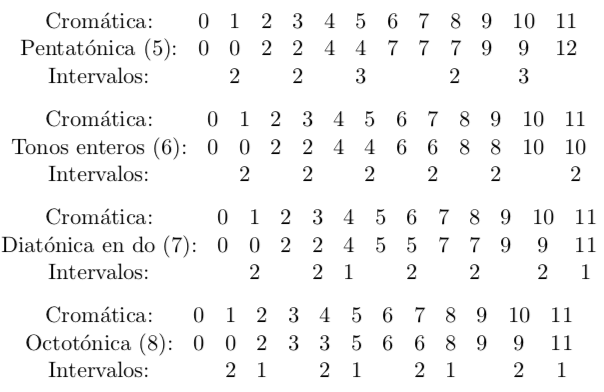
\includegraphics[width=12cm]{Fotos/Re-escalando-musica-fig-3.png}
\end{center}

%\[\left.\begin{array}{*{13}c}
%\text{Crom�tica:}&0&1&2&3&4&5&6&7&8&9&10&11\\
%\text{Pentat�nica (5):}&0&0&2&2&4&4&7&7&7&9&9&12\\
%\text{Intervalos:}&&2&&2&&3&&&2&&3&\\
%\end{array}\right.\]		
%\[\left.\begin{array}{*{13}c}
%\text{Crom�tica:}&0&1&2&3&4&5&6&7&8&9&10&11\\
%\text{Tonos enteros (6):}&0&0&2&2&4&4&6&6&8&8&10&10\\
%\text{Intervalos:}&&2&&2&&2&&2&&2&&2\\
%\end{array}\right.\]
%\[\left.\begin{array}{*{13}c}
%\text{Crom�tica:}&0&1&2&3&4&5&6&7&8&9&10&11\\
%\text{Diat�nica en do (7):}&0&0&2&2&4&5&5&7&7&9&9&11\\
%\text{Intervalos:}&&2&&2&1&&2&&2&&2&1\\
%\end{array}\right.\]        
%\[\left.\begin{array}{*{13}c}
%\text{Crom�tica:}&0&1&2&3&4&5&6&7&8&9&10&11\\
%\text{Octot�nica (8):}&0&0&2&3&3&5&6&6&8&9&9&11\\
%\text{Intervalos:}&&2&1&&2&1&&2&1&&2&1\\
%\end{array}\right.\]

	\subsection{Obras modificadas}
	
	Ahora se describir�n las obras que pasar�n por la modificaci�n. Para abarcar distintos estilos compositivos y hacer este estudio m�s amplio, he escogido obras de los tres principales compositores dodecaf�nicos: Schoenberg, Berg y Webern.
	
	Sin embargo, no se han escogido obras de compositores posteriores ni serialistas integrales. Uno de los motivos es porque interesa en este estudio la relaci�n entre los sonidos: no se modifican m�s que las alturas de las notas, y por tanto no se tiene en cuenta el resto de elementos musicales. Que est�n compuestos serialmente no afecta a las conclusiones de este experimento.
	
	Por otro lado, los compositores posteriores a Schoenberg todav�a no han pasado al dominio p�blico. Eso impide, por desgracia, que se pueda trabajar libremente con su m�sica.
	
	Por �ltimo, el hecho de que cada nota tenga su propia din�mica, su propia articulaci�n o su propio timbre hace de las obras serialistas integrales dif�ciles de manipular. Adem�s, como los audios est�n hechos mediante ordenador y no con int�rpretes reales, la calidad y la intenci�n musical de estas partituras tan complicadas nunca podr�an plasmarse a la perfecci�n.
	
	La primera obra que pasar� por el algoritmo de modificaci�n serial es la \textit{Suite para piano}, Op. 25 de Schoenberg. Un an�lisis de esta pieza y de su contexto hist�rico se puede encontrar en \cite{celia1}.
	
	Su \href{http://www.ccarh.org/publications/data/humdrum/tonerow/files/schoenberg/schoenberg04.pc.krn}{serie principal} es: 
	\begin{center}
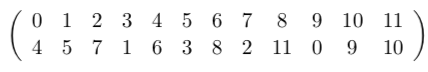
\includegraphics[width=7.5cm]{Fotos/Re-escalando-musica-fig-4.png}
\end{center}

%	\drow{4,5,7,1,6,3,8,2,11,0,9,10}

	\begin{center}
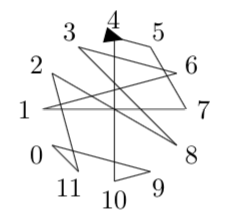
\includegraphics[width=4cm]{Fotos/Re-escalando-musica-fig-5.png}
\end{center}

%\begin{center}
%		\ddiagram{4,5,7,1,6,3,8,2,11,0,9,10}
%\end{center}
	
	La segunda obra es un arreglo para soprano y piano de una de las arias m�s destacadas de la segunda �pera de Alban Berg, \textit{Lulu}. El libreto de la obra est� basado en dos tragedias de Frank Wedekind: ``El esp�ritu de la tierra'' y ``La Caja de Pandora''.
	
	El aria, llamada \textit{Lied der Lulu}, es parte de una dram�tica disputa entre Lulu y su marido por las infidelidades de ella, que acaba con el homicidio accidental de �l.
	
	La \href{http://www.ccarh.org/publications/data/humdrum/tonerow/files/berg/berg10.pc.krn}{serie} de Lulu es:
	\begin{center}
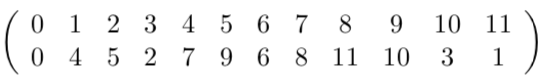
\includegraphics[width=7.5cm]{Fotos/Re-escalando-musica-fig-6.png}
\end{center}

%		\drow{0,4,5,2,7,9,6,8,11,10,3,1}
	\begin{center}
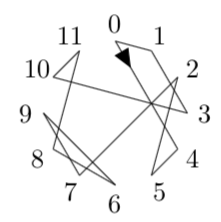
\includegraphics[width=4cm]{Fotos/Re-escalando-musica-fig-7.png}
\end{center}
%\begin{center}
%		\ddiagram{0,4,5,2,7,9,6,8,11,10,3,1}
%\end{center}
	
	La tercera, de 1936, es la �nica obra publicada de Anton Webern para piano solo: \textit{Variationen f�r Klavier}, Op. 27, y se compone de tres movimientos: \textit{Sehr m�ssig}, \textit{Sehr schnell} y \textit{Ruhig fliessend}.
	
	Su \href{http://www.ccarh.org/publications/data/humdrum/tonerow/files/webern/webern17.pc.krn}{serie principal} es:
		\begin{center}
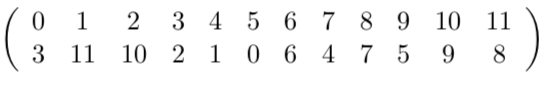
\includegraphics[width=7.5cm]{Fotos/Re-escalando-musica-fig-8.png}
\end{center}
%		\drow{3,11,10,2,1,0,6,4,7,5,9,8}
	\begin{center}
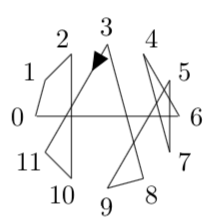
\includegraphics[width=4cm]{Fotos/Re-escalando-musica-fig-9.png}
\end{center}
%\begin{center}
%		\ddiagram{3,11,10,2,1,0,6,4,7,5,9,8}
%\end{center}
    
    \subsection{Programa \textit{online} de modificaci�n de partituras}
	He creado una p�gina web \textit{online} que transforma cada nota de una partitura a cualquier nota requerida, una a una. Este \textit{software} sirve para no tener que modificar a mano las partituras del experimento, pero tambi�n puede servir para otros prop�sitos. Por ejemplo, para cambiar una partitura de mayor a menor, o viceversa.
	
	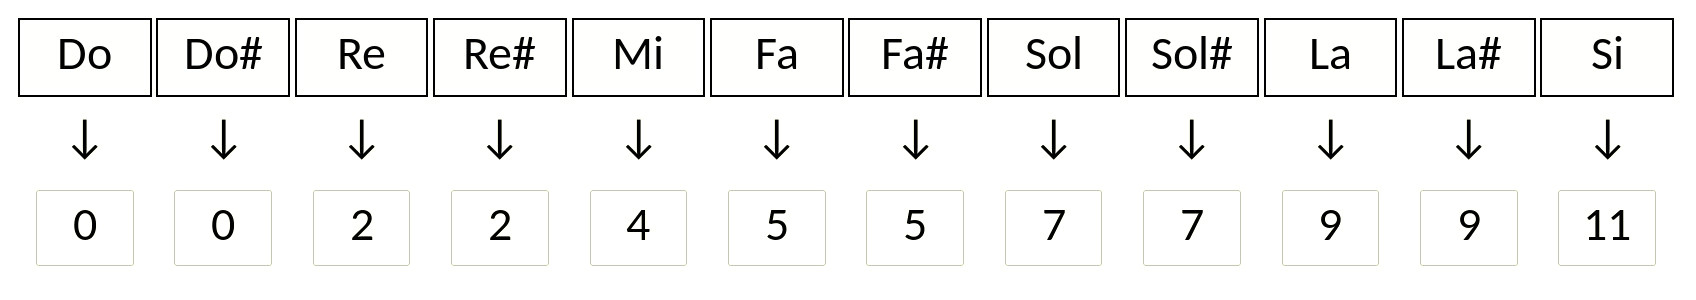
\includegraphics[width=15cm]{whiteweb2.jpg}
	
	El programa solo admite partituras con formato \textit{Archivo Musescore sin Comprimir} (\textit{.mscx}) del software libre \href{https://musescore.org/}{\textit{Musescore}}. En caso de tener la partitura en otro formato, debe abrirse en \textit{Musescore} y guardarse en el formato correcto. Est� escrita en Elm y el c�digo puede encontrarse \href{https://gitlab.com/dodecafonismo/modificaciones}{aqu�}.
	
   	 La aplicaci�n web se encuentra en el siguiente enlace: \url{https://modificaciones.netlify.com/}. Sus instrucciones de uso se encuentran al final de la p�gina web.
    
    \section{Conclusiones}
    Todas las conclusiones que se pueden extraer de este experimento son enteramente subjetivas. El objetivo de realizarlo es poder seguir investigando con las propiedades matem�ticas de la m�sica, y analizar el impacto emocional que estas pueden causar.
    
    No se puede afirmar que la transformaci�n mejore o empeore ninguna obra. En todo caso podemos interpretar qu� transformaciones tienen un determinado sentido musical o est�tico, dependiendo de la escala utilizada o del estilo con el que est�n compuestas.     
    Tampoco debemos olvidar que el cromatismo siempre aportar� a las obras una dimensi�n a�adida, un elemento extra que ha impulsado gran parte de la innovaci�n en la historia de la m�sica. Quitarlo por completo es, en realidad, retroceder en la evoluci�n del arte.
   	
   	En general, las transformaciones hexat�nica (6) y octot�nica (8) siguen conservando mucho del cromatismo que tiene la partitura original. Siguen sonando ajenas al o�do tonal del oyente medio. Vamos a comentar algunas de las impresiones que generan las otras dos transformaciones en cada una de las obras, aunque dejaremos al lector que forme su propia opini�n.
   	
    \subsection{Obra de Berg: Lied der Lulu}
	El estilo compositivo de Berg busca, en su mayor parte, acercarse a las formas tonales; maneja la falta de tonalidad serialista sin deshacerse de muchos elementos de la tradici�n musical. Sus melod�as son fluidas y su fraseo inicia a conversar. As�, la transformaci�n pentat�nica (5) queda, quiz�s, algo simplista y repetitiva, y es en cambio la heptat�nica (7) la que nos traslada a sonoridades m�s familiares.
	
    \url{https://soundcloud.com/celiarubio/sets/berg-lied-der-lulu}
    
    \subsection{Obra de Webern: Variationen op. 27}
    El estilo compositivo de Webern es rompedor y enigm�tico. Tanto fue as� que su m�sica sirvi� de inspiraci�n para el serialismo integral de los a�os 50. Sus melod�as suenan fragmentadas y est�n llenas de intervalos de m�s de una octava. Es, por tanto, muy dif�cil que cualquier transformaci�n que conserve similitudes mel�dicas con la partitura original pueda acercarse a m�sicas m�s convencionales. La esencia de esta obra est� precisamente en su peculiaridad.
    
    \url{https://soundcloud.com/celiarubio/sets/webern-op27-variations}
    
    
    \subsection{Obra de Schoenberg: Suite op. 25}
    El estilo compositivo de Schoenberg en la Suite es tradicional, aunque busca nuevas sonoridades. Su principal objetivo es conservar la estructura formal anterior, y por ello lo �nico que aleja a la obra es el uso del serialismo en la altura de las notas.
    
    La obra es, en general, m�s arm�nica que mel�dica, ya que pretende simular texturas instrumentales del periodo barroco. Adem�s, al centrarse tanto en la formalidad de la pieza aporta una riqueza separada del uso del serialismo. Por ello, la transformaci�n pentat�nica (5) no acaba siendo mon�tona sino muy sugestiva.
    
    Por otro lado, la elecci�n concreta de la funci�n transformativa, que hace predominar las notas do y sol \textemdash que aparecen en la nueva serie una vez m�s que el resto de notas\textemdash~provoca que, en muchos casos, la obra simule estar en do mayor. Como en la partitura original predomina el intervalo de tritono re $\flat$ \textendash~sol, la transformaci�n da peso al intervalo de quinta justa, que es la base de la armon�a tradicional.
    
    La transformaci�n heptat�nica (7) sigue dejando alguna disonancia debido a la existencia de semitonos entre las notas mi \textendash~fa y si \textendash~do, y al tritono en fa \textendash~si. Al ser una obra ampliamente textural, muchos de estos intervalos aparecen con frecuencia.
    
    \url{https://soundcloud.com/celiarubio/sets/schoenberg-op25-1-prelude}
    
    \url{https://soundcloud.com/celiarubio/sets/schoenberg-op25-2a-gavotte}
    
    \url{https://soundcloud.com/celiarubio/sets/schoenberg-op25-2b-musette}
    
    \url{https://soundcloud.com/celiarubio/sets/schoenberg-op25-3-intermezzo}
    
    \url{https://soundcloud.com/celiarubio/sets/schoenberg-op25-4a-menuet}
    
    \url{https://soundcloud.com/celiarubio/sets/schoenberg-op25-4b-trio}
    
    \url{https://soundcloud.com/celiarubio/sets/schoenberg-op25-5-gigue}

	
\bibliographystyle{plain}
\bibliography{Re-escalando-musica.bib}
\end{document}





